%----------------------------------------------------------------------------------------
%	PACKAGES AND DOCUMENT CONFIGURATIONS
%----------------------------------------------------------------------------------------

\documentclass{article}


\usepackage{graphicx} % Required for the inclusion of images
\graphicspath{{figures/}}
\usepackage{subfigure} % Required for the inclusion of images
\usepackage{natbib} % Required to change bibliography style to APA
\usepackage{amsmath} % Required for some math elements 
\usepackage{listings}
\usepackage{xcolor}
\usepackage{fontspec}
\usepackage{ctex}
\usepackage{geometry}
\geometry{a4paper,scale=0.8}
\renewcommand{\contentsname}{\centerline{目录}}
\setmonofont{Consolas}
\lstset{
basicstyle=\ttfamily\footnotesize,%
escapeinside=``,%
keywordstyle=\color{black},%\bfseries, \underbar,%
identifierstyle={},%
tabsize=4,
commentstyle=\color{blue},%
stringstyle=\ttfamily,%
%labelstyle=\tiny,%
extendedchars=false,%
linewidth=\textwidth,%
numbers=left,%
numberstyle=\tiny \color{blue},%
frame=trbl%
}
%点列
%\begin{itemize}
%\item[$\bullet$]Get familiar with Y86 assembly language.
%\end{itemize}

%小标题
%\begin{center}
%{\ttfamily rsum.ys}
%\end{center}
%代码
%\begin{lstlisting}[language={[ANSI]C}]
%\end{lstlisting}
%点列和浮动体图表和ref
%\begin{itemize}
%\item[$\bullet$]{\ttfamily sum.ys} (Figure \ref{Part A: sum.ys})\\
%\end{itemize}
%\begin{figure}[htbp]%figure浮动体环境 [htbp]指定位置
%		\centering%居中排版
%		\includegraphics{A_sum}
%		\caption{Part A  {\ttfamily sum.ys}} \label{Part A: sum.ys}%标题 自动编号 label标签
%\end{figure}


%\usepackage{times} % Uncomment to use the Times New Roman font

%----------------------------------------------------------------------------------------
%	DOCUMENT INFORMATION
%----------------------------------------------------------------------------------------

\title{\textbf{操作系统课程设计Project 6\\Banker's Algorithm}} % Title

\author{姓名: 郭倩昀  
\\班级: F1903303  
\\学号: 519021910095  
\\Email: guoqianyun@sjtu.edu.cn} % Author name and email
\date{\today} % Date for the report
\begin{document}
\maketitle % Insert the title, author and date
\tableofcontents
\newpage
\section{Banker's Algorithm}
\subsection{实验内容与目标}
本实验需要利用C语言实现银行家算法,支持功能如下:
\begin{itemize}
\item[$\bullet$]支持指令RQ来为进程申请资源
\item[$\bullet$]支持指令RL来释放进程的资源
\item[$\bullet$]支持指令*来输出当前资源分配状态
\item[$\bullet$]支持指令EXIT退出运行
\end{itemize}
\subsection{实验过程及步骤}
\begin{itemize}
\item[$\bullet$]设计全局变量\\
将银行家算法最基本的变量设计为全局变量,包括资源数,进程数,available矩阵,maximum矩阵,allocation矩阵以及need矩阵。
\item[$\bullet$]数据初始化\\
根据执行命令可以得出资源数,初始化available矩阵。进程数以及maximum矩阵的初始化需要读取maximum.txt文件获得,初始化过程中由于进程数位置,要注意空间的分配。
\item[$\bullet$]指令分析\\
设计函数parse\_inst标准化处理buffer中输入的指令,将指令操作存入op,指令数据存入args。
\item[$\bullet$]更新need矩阵\\
由于算法中分配情况不同时都要及时更新need矩阵,将该步骤包裹为update\_need函数,need矩阵根据目前的maximum矩阵和allocation矩阵信息重新计算。
\item[$\bullet$]RQ申请资源\\
设计request\_resources函数完成用户进程资源分配工作。首先要检查用户进程的针对每一个资源的申请数量是否大于用户进程所需的最大数量或者目前可用资源的数量,如果超出则打印相应错误并退出。之后创建临时的available矩阵假设接受资源申请并判断状态是否安全。每次选取一个没有被服务的进程查看是否可以分配最大需求资源并服务完成,如果可以那么就回收其目前所属资源并记录已被服务,如果有未被服务的用户进程但是都没法分配最大需求资源,说明当前状态不安全,需要拒绝该申请,收回分配的资源。若状态安全,就更新所有的矩阵信息表示接受申请并已经分配资源。
\item[$\bullet$]RL释放资源\\
设计release\_resources函数完成用户进程资源释放工作。首先要检查用户进程的针对每一个资源的释放数量是否大于该进程所拥有的资源数量,如果超出则打印相应错误并退出。若可以正常释放,更新相关矩阵信息并输出成功释放的信息。
\item[$\bullet$]*打印状态\\
设计print\_value打印当前状态,并传入打印选项,若参数为0则打印available,maximum和资源数进程数信息;若参数为1则另外打印allocation信息;若参数为2则另外打印need信息。
\item[$\bullet$]main()函数设计\\
main()函数需要把所有已设计的函数和功能连接起来,首先初始化所有数据,然后需要检查当前状态是否安全(是否可用资源数都大于进程最大需求资源数),如果不安全需要报错退出。读入指令并分析指令,指令不合法需要报错退出,然后根据指令类型调用相应的申请资源、释放资源的函数,最后要即使释放先前分配的的空间。
\end{itemize}
\subsection{实验代码}
\begin{center}
{\ttfamily banker.c}
\end{center}
\begin{lstlisting}[language={[ANSI]C}]
# include <stdio.h>
# include <stdlib.h>
# include <string.h>
# include <unistd.h>
# define MAX_LINE 500
# define TRUE 1
int resource_num;
int customer_num;

int *available;		// the available amount of each resource
int **maximum;		// the maximum demand of each customer
int **allocation;	// the amount currently allocated to each other
int **need;			// the remaining need of each customer

void initialize(int argc, char *argv[]);
int parse_inst(char *buf, char *op, int *argn, int *arg);	//Parse the buffer
void update_need(int ** need, int ** maximum, int ** allocation);	//Update the need
int request_resources(int customer_id, int request[]);		//Request the resources
void release_resources(int customer_id, int release[]);		//Release the resources
void print_value(int printop);								//* print current value


int main(int argc, char *argv[]) {

//Initialize the arrays
	initialize(argc, argv);
	
//print initial state
	print_value(0);
	
// Check whether the initial state is safe
	static int err=0;
	for (int i = 0; i < customer_num; ++ i)
	{
		for (int j = 0; j < resource_num; ++ j)
			{
				if(maximum[i][j] > available[j]) 
				{err=1;}
			}
	}
	if (err) {
		fprintf(stdout, "  ERROR: Initial state is unsafe\n");
		exit(1);
	}
	
//read in inst
	char buf[MAX_LINE], op[MAX_LINE];
	int *arg = (int *) malloc (sizeof(int) * (1 + resource_num));
	int argn;

	while(TRUE) 
	{
		fprintf(stdout, "Banker >> ");
		fgets(buf, MAX_LINE, stdin);
		
		//Parse the buffer to op and arg
		err = parse_inst(buf, op, &argn, arg);
		if (err) {
			fprintf(stdout, "  ERROR: Invalid instruction\n");
			continue;
		}
		
		//op
		if (strcmp(op, "EXIT") == 0 && argn == 0)//end
			break;
		else if (strcmp(op, "*") == 0 && argn == 0)//print current value
			print_value(2);
		else if (strcmp(op, "RQ") == 0 && argn == resource_num + 1) 
		{
			if (request_resources(arg[0], arg + 1)==-1)	//unsafe
				fprintf(stdout, "  Request command denied.\n");
			else									//safe
				fprintf(stdout, "  Request command accepted.\n");
		}
		else if (strcmp(op, "RL") == 0 && argn == resource_num + 1)//release
			release_resources(arg[0], arg + 1);
		else 
		{
			fprintf(stdout, "  ERROR: Invalid instruction\n");
			continue;
		}
	}
//free
	free(arg);
	free(available);
	for (int i = 0; i < customer_num; ++ i) 
	{
		free(maximum[i]);
		free(allocation[i]);
		free(need[i]);
	}
	free(maximum);
	free(allocation);
	free(need);
	return 0;
}

//Initialize the arrays
void initialize(int argc, char *argv[]) {
	//read in resources
	resource_num = argc - 1;
	if (resource_num == 0) 
	{
		fprintf(stderr, "  ERROR: no resource!\n");
		exit(1);
	}
	//initialize available
	available = (int *) malloc (sizeof(int) * resource_num);
	for (int i = 1; i < argc; ++ i)
		available[i - 1] = atoi(argv[i]);

	//initialize customer maximum
	customer_num = 0;
	int capacity = 100;//default capacity
	maximum = (int **) malloc (sizeof(int *) * capacity);

	//read data from maximum.txt
	FILE *fp = fopen("maximum.txt", "r");
	static int data;
	while(fscanf(fp, "%d", &data)!=EOF)
	{
		//double the array if full
		if (customer_num == capacity) 
		{
			int ** tmp;
			tmp = (int **) malloc (sizeof(int *) * capacity * 2);
			for (int i = 0; i < capacity; ++ i) 
			{
				tmp[i] = (int *) malloc (sizeof(int) * resource_num);
				for (int j = 0; j < resource_num; ++ j)
					tmp[i][j] = maximum[i][j];
				free(maximum[i]);
			}
			free(maximum);
			maximum = tmp;
			capacity*=2;
		}
		
		// read the data
		maximum[customer_num] = (int *) malloc (sizeof(int) * resource_num);
		maximum[customer_num][0] = data;
		for (int i = 1; i < resource_num; ++ i)
		{
			fscanf(fp, ",%d", &data);
			maximum[customer_num][i] = data;
		}
		customer_num ++;
	}
	fclose(fp);
	
	//initialize allocation
	allocation = (int **) malloc (sizeof(int *) * capacity);
	for (int i = 0; i < customer_num; ++ i)
		allocation[i] = (int *) malloc (sizeof(int) * resource_num);
		
	for (int i = 0; i < customer_num; ++ i)
		for (int j = 0; j < resource_num; ++ j) 
			allocation[i][j] = 0;
			
	//initialize need
	need = (int **) malloc (sizeof(int *) * capacity);
	for (int i = 0; i < customer_num; ++ i)
		need[i] = (int *) malloc (sizeof(int) * resource_num);
	update_need(need, maximum, allocation);
}

//Update need
void update_need(int **need, int **maximum, int **allocation)
{
	for (int i = 0; i < customer_num; ++ i)
		for (int j = 0; j < resource_num; ++ j)
			need[i][j] = maximum[i][j] - allocation[i][j];
}

//Parse the buffer
int parse_inst(char *buf, char *op, int *argn, int *arg)
{
	int last_blank=1;
	int tmp=0;
	int opdex = 0;	
	(*argn) = -1;	
	for (int i = 0; buf[i]; ++ i) 
	{
		if (buf[i] == ' ' || buf[i] == '\t' || buf[i] == '\n') 
		{
			if (last_blank) continue;
			last_blank = 1;
			if (*argn != -1) //data
			{
				if (*argn == resource_num + 1) return 1;
				arg[*argn] = tmp;
				tmp = 0;//renew tmp
			}
			(*argn) ++;
		} 
		else 
		{
			last_blank = 0;
			if(*argn == -1) //op
				op[opdex++] = buf[i];
			else 			//data
			{
				if (buf[i]>='0' && buf[i]<='9') tmp = tmp*10+buf[i]-'0';
				else return 1;
			}
		}
	}
	op[opdex] = 0;
	if(!last_blank) //check buffer end
	{
		if (*argn != -1) 
		{
			if (*argn == resource_num + 1) return 1;				
			arg[*argn] = tmp;
			tmp = 0;//renew tmp
		}
		(*argn) ++;
	}
	return 0;	
}

// Request the resources
int request_resources(int customer_id, int request[])
{
	//pre-check
	for (int i = 0; i < resource_num; ++ i)
		if (request[i] > need[customer_id][i]) 
		{
			fprintf(stdout, "  ERROR: The request is greater than need\n");
			return -1;
		}
	for (int i = 0; i < resource_num; ++ i)
		if (request[i] > available[i]) 
		{
			fprintf(stdout, "  ERROR: Not enough available resources\n");
			return -1;
		}
	
	//grant the request
	int *available_tmp;
	int *is_served;
	available_tmp = (int *) malloc (sizeof(int) * resource_num);
	is_served = (int *) malloc (sizeof(int) * customer_num);
	for (int i = 0; i < customer_num; ++ i)
		is_served[i] = 0;
	for (int i = 0; i < resource_num; ++ i) {
		available_tmp[i] = available[i] - request[i];
		allocation[customer_id][i] += request[i];
	}
	update_need(need, maximum, allocation);
	
	//check
	int safe = 1;
	for (int step = 0; step < customer_num; ++ step) {
		//Find next customer	
		int dex = -1;
		for (int i = 0; i < customer_num; ++ i) 
		{
			if (is_served[i]) continue;
			int flag = 1;
			for (int j = 0; j < resource_num; ++ j)
				if (need[i][j] > available_tmp[j]) 
				{
					flag = 0;
					break;
				}
			if (flag) 
			{
				dex = i;
				break;
			}
		}
		//Not found, unsafe.
		if(dex == -1) {
			safe = 0;
			break;
		}
		//Found, serve the customer.
		is_served[dex] = 1;
		for (int i = 0; i < resource_num; ++ i)
			available_tmp[i] += allocation[dex][i];
	}
	
	//safe
	if (safe) 
	{
		fprintf(stdout, "  Request is granted.\n");
		for (int i = 0; i < resource_num; ++ i)
			available[i] -= request[i];					//grant the request
		free(available_tmp);
		free(is_served);
		return 0;
	} 
	else 
	{
		fprintf(stdout, "  Unsafe state, request CANNOT be granted\n");
		for (int i = 0; i < resource_num; ++ i)
			allocation[customer_id][i] -= request[i];	//take back the resourses
		update_need(need, maximum, allocation);
		free(available_tmp);
		free(is_served);
		return -1;
	}
}

// Release the resources
void release_resources(int customer_id, int release[])
{
	//Pre-Check
	for (int i = 0; i < resource_num; ++ i)
		if (release[i] > allocation[customer_id][i]) 
		{
			fprintf(stdout, "  ERROR: The release is greater than allocation\n");
			return;
		}
		
	//update available and allocation
	for (int i = 0; i < resource_num; ++ i) {
		available[i] += release[i];
		allocation[customer_id][i] -= release[i];
	}
	update_need(need, maximum, allocation);
	fprintf(stdout, "  The resources are released.\n");
	return;
}

//* print current value
//printop 0 available maximum
//printop 1 available maximum allocation
//printop 2 available maximum allocation need
void print_value(int printop)
{
	fprintf(stdout, "Current State: \n");
	fprintf(stdout, "  Customer Number = %d\n  Resource Number = %d\n", customer_num, resource_num);
	
	//available
	fprintf(stdout, "  Available = [");
	for (int i = 0; i < resource_num; ++ i)
		{
			fprintf(stdout, "%d", available[i]);
			if(i == resource_num - 1) fprintf(stdout,"]\n");
			else  fprintf(stdout,", ");
		}
	//maximum
	fprintf(stdout, "  Maximum = \n");
	for (int i = 0; i < customer_num; ++ i) {
		fprintf(stdout, "    [");
		for (int j = 0; j < resource_num; ++ j)
		{
			fprintf(stdout, "%d", maximum[i][j]);
			if(j == resource_num - 1) fprintf(stdout,"]\n");
			else  fprintf(stdout,", ");
		}
	}

	//allocation
	if (printop >= 1) {
		fprintf(stdout, "  Allocation = \n");
		for (int i = 0; i < customer_num; ++ i) {
			fprintf(stdout, "    [");
			for (int j = 0; j < resource_num; ++ j)
			{
				fprintf(stdout, "%d", allocation[i][j]);
				if(j == resource_num - 1) fprintf(stdout,"]\n");
				else  fprintf(stdout,", ");
			}
		}
	}
	
	//need
	if (printop >= 2) {
		fprintf(stdout, "  Need = \n");
		for (int i = 0; i < customer_num; ++ i) {
			fprintf(stdout, "    [");
			for (int j = 0; j < resource_num; ++ j)
			{
				fprintf(stdout, "%d", need[i][j]);
				if(j == resource_num - 1) fprintf(stdout,"]\n");
				else  fprintf(stdout,", ");
			}
		}
	}
}
\end{lstlisting}
\begin{center}
{\ttfamily maximum.txt}
\end{center}
\begin{lstlisting}[language={[ANSI]C}]
6,4,7,3
4,2,3,2
2,5,3,3
6,3,3,2
5,6,7,5
\end{lstlisting}
\subsection{实验测试}
\begin{itemize}
\item[$\bullet$]banker测试
测试指令如下
\begin{lstlisting}[language={[ANSI]C}]
make
./banker 10 4 9 7
./banker 10 6 9 7
RQ 0 6 4 7 3
*
RQ 1 5 2 2 2
RQ 1 4 2 2 2
RQ 4 0 0 0 1
RL 0 1 1 1 3
RQ 4 1 1 1 1
*
EXIT
\end{lstlisting}
首先用Makefile文件编译,生成可执行文件banker,然后输入资源数10 4 9 7并执行,发现初始状态不安全,报错并退出(如图 \ref{banker测试1})。然后输入资源数10 6 9 7并执行,RQ 0 6 4 7 3申请资源分配成功;输入*打印状态;输入RQ 1 5 2 2 2申请资源发现申请数量超出所需,报错并拒绝请求;RQ 1 4 2 2 2和RQ 4 0 0 0 1申请资源分配成功;RL 0 1 1 1 3释放资源成功;RQ 4 1 1 1 1申请资源发现状态不安全,报错并拒绝请求;输入*打印状态;最后输入EXIT退出运行。
\end{itemize}
\begin{figure}[htbp]
		\centering
		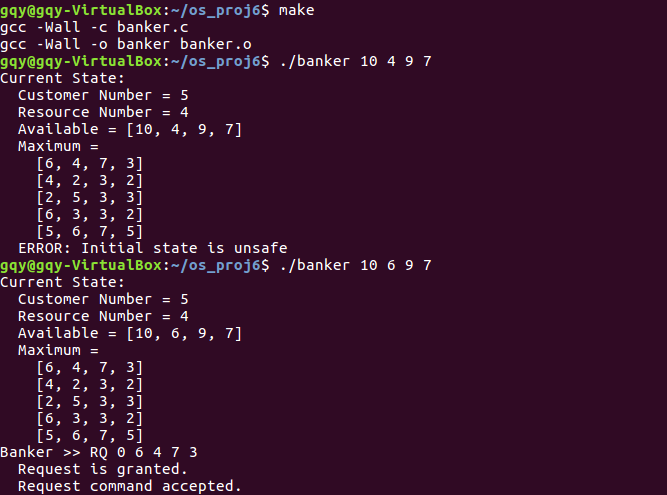
\includegraphics{b1}
		\caption{banker测试1} \label{banker测试1}
\end{figure}
\begin{figure}[htbp]
		\centering
		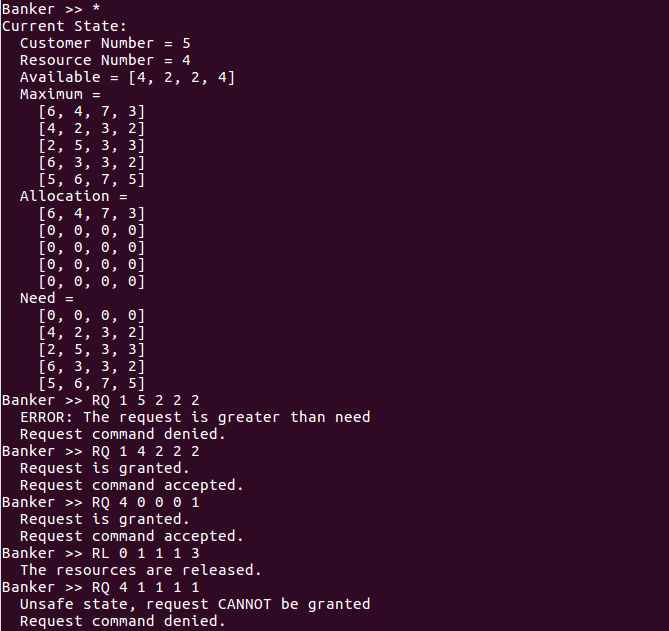
\includegraphics{b2}
		\caption{banker测试2} \label{banker测试2}
\end{figure}
\begin{figure}[htbp]
		\centering
		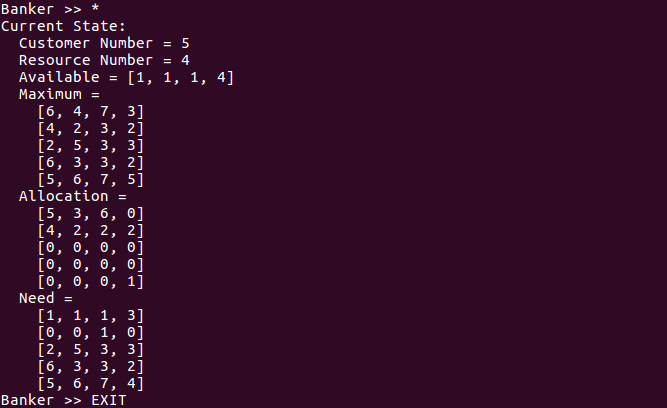
\includegraphics{b3}
		\caption{banker测试3} \label{banker测试3}
\end{figure}
\section{Conclusion}

\subsection{问题与解决方案}
本次project6对银行家算法的实现难度并不大,设计思路比较清晰,按部就班完成各部分函数设计支持几类指令就可以顺利完成,主要难点在于用户资源申请资源分配的时候安全状态的检查,以及每次状态变化的时候数据信息的更新维护要仔细编程,还有需要考虑多种非法的特殊情况,及时报错退出。

\subsection{实验心得}
本次project6将进程资源管理的经典算法银行家算法顺利实现,是对所学知识一次很透彻的运用,在锻炼了程序设计能力的同时加深了对理论知识的理解,完成整体算法设计的实现也让我非常有成就感,总体来说让我收获颇丰。

%----------------------------------------------------------------------------------------


\end{document}